\documentclass[12pt]{article}

\usepackage{sbc-template}
\usepackage{graphicx,url}

\usepackage[brazil]{babel}
%\usepackage[latin1]{inputenc}
\usepackage[utf8]{inputenc}
% UTF-8 encoding is recommended by ShareLaTex

\newcommand\ceil[1]{\lceil#1\rceil}
\usepackage{relsize}

\sloppy

\title{Aplicação de Redes Neurais Artificiais no Mercado de Ações}

\author{Thiago V. de A. Silva\inst{1} }


\address{Departamento de Ciência da Computação \\
  Universidade Federal de Minas Gerais\\
  31270-010 -- Belo Horizonte -- MG -- Brasil
  \email{thiagovieiraas@gmail.com.br}
}

\begin{document} 

\maketitle

%TODO: A Good abstract
\iffalse
\begin{resumo}
\end{resumo}

\begin{abstract}
\end{abstract}
\fi

\section{Introdução}

O objetivo deste trabalho é avaliar um conjunto de redes neurais, e elaborar uma estratégia de negociação de papéis de ações. Os resultados serão analisados em termos estatísticos e financeiros. Para a análise estatística, variáveis como quantidade de acertos e erros nas previsões das redes neurais serão levadas em conta; na análise financeira, as redes neurais serão aplicadas em simulações usando dados históricos de ativos da BOVESPA.

\section{Metodologia} \label{sec:firstpage}

\subsection{Conjunto de Dados}
Do conjuntos de empresas listadas na BOVESPA, cinco foram escolhidas para serem usadas como base de dados para treinamentos e testes das redes neurais, além do índice Ibovespa. %Falar do intervalo de tempo considerado nos testes.
Os ativos selecionados para a realização deste trabalho são:
\begin{enumerate}
\item BOVA11
\item ITUB4
\item CIEL3
\item ABEV3
\item CMIG4
\item EMBR3
\end{enumerate}

A escolha dos ativos foi baseada principalmente no fato das empresas terem setores de atuação diferentes, sendo eles financeiro, consumo não-cíclico, utilidade pública e bens industriais.

\subsection{Definição do Modelos das Rede Neurais}
% Multilayer Perceptron - Feedforward - Calibragem - Backprop
% Numero de nós na hidden layer - sqrt(input+output) seguindo o paper do conegundes
%TODO: Falar da função de ativação também

Várias redes neurais com inputs diferentes serão geradas, todas elas serão redes \emph{multi-layer perceptrons} e serão treinadas usando o algoritmo de treinamento \emph{backpropagation}. O número de nós na camada escondida será dado por $\ceil{\frac{(I+O)}{2}}$ , onde I é o número de vértices do input e O é o número de vértices do output.

% Colocar uma imagem da rede neural aqui...
\begin{center}
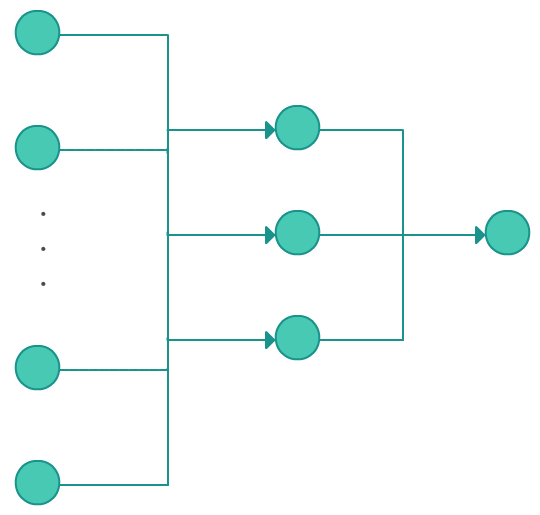
\includegraphics[scale=0.45]{gg}\\
\emph{Figura 1: Exemplo de Rede Neural Artificial}\\
\end{center}

A função de ativação é uma sigmóide definida por: \\
\begin{center}
$\mathlarger{S(t) = \frac{2}{1+e^t}-1}$
\end{center}
\subsubsection{Entrada}
As variáveis a serem consideradas como input são:
\begin{enumerate}
\item O preço de fechamento dos últimos x dias.
\item O preço de abertura dos últimos x dias.
\item O preço máximo diário dos últimos x dias.
\item O preço mínimo diário dos últimos x dias.
\item Média móvel simples (MMS) do preço de fechamento dos últimos x dias.
\item Média móvel exponencial (MME) do preço de fechamento dos últimos x dias.
\item Proporção definida por $\frac{MME}{MMS}$ dos últimos x dias.
\item Bollinger Bands.
\item MACD.
\end{enumerate}

Cada rede neural criada terá um subconjuntos das variáveis apresentadas acima. Os valores de x são fixados em 5, 7, 10 ou 15 dias em cada configuração da rede neural.

\subsubsection{Saída}
A saída da rede neural estará no intervalo [-1,1], onde -1 indicará um possível movimento de queda, e 1 indicará um possível movimento de alta.

\subsubsection{Treinamento e Testes}
Os treinamentos serão feitos usando o algoritmo de \emph{backpropagation}. Para treinar as redes neurais, irei utilizar os dados históricos dos ativos desde 1 de janeiro de 2012 à 1 de janeiro de 2013.\\
Serão executados vários testes, seguindo uma janela deslizante pelo intervalo de tempo definido acima. A cada 2x dias, os primeiros x dias da janela serão usados para treinamento e os x dias seguintes serão usados para teste.
%\subsection{Caracterização dos Dados}

\end{document}
